\chapter{项目特色}
\section{数据库连接池}
\subsection{背景}

\subsubsection{原始JDBC连接缺陷}
在项目一和项目三中,连接数据库的方式是传统的JDBC连接。每进行一次SQL操作就需要经过创建连接,操作,释放连接的步骤,所有连接都是临时短暂的。

\subsubsection{出现问题}
Mysql 查询大量数据异常:

默认情况下,Windows允许用于使用5000个临时TCP端口。任何端口关闭后,它将在TIME WAIT状态保持120秒。与重新初始化全新的连接相比,该状态允许以更低的开销重新使用连接。但是,在该时间逝去前,无法再次使用该端口。

如果TCP端口堆栈较少,以及具有TIME WAIT状态的大量在短时间内打开和关闭的 TCP端口,就很可能遇到端口耗尽问题。

\subsection{优化方法}
连接池技术:一种池化技术。在程序第一次启动的时候,程序会初始化连接池,连接池里面存放的是连接Mysql数据库的连接,并且统一管理释放。当有线程需要进行SQL操作时,他会从线程池里取一个连接,
操作完成之后将连接归还回连接池。这样就将短命临时的数据库连接变成了持久性的连接,有效地解决了临时端口消耗过快,后端与数据库连接消耗过多时间的问题。

\subsection{使用效果}

压力测试:查看连续进行10000次SQL搜索的时间

采用连接池前:
\begin{figure}[htbp]
	\centering
	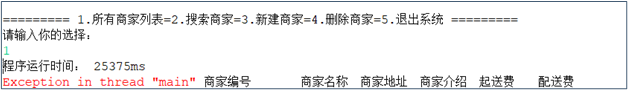
\includegraphics[width=0.8\textwidth]{lianjiechia}
	\caption{优化后}
	\vspace{\baselineskip}
\end{figure}

 
采用连接池后:
\begin{figure}[htbp]
	\centering
	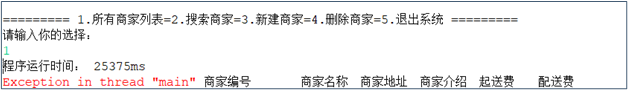
\includegraphics[width=0.8\textwidth]{lianjiechia}
	\caption{优化后}
	\vspace{\baselineskip}
\end{figure}
\section{数据库缓存}
\subsection{背景}

当网站的处理和访问量非常大的时候,数据库的压力就变大了,数据库的连接池,数据库同时处理数据的能力就会受到很大的挑战,一旦数据库承受了其最大承受能力,网站的数据处理效率就会大打折扣。

\subsection{技术原理}
Redis其实就是说把表中经常访问的记录放在了Redis中,然后用户查询时先去查询Redis再去查询MySQL,确实实现了读写分离,也就是Redis只做读操作。由于缓存在内存中,所以查询会很快。

同时还需注意数据库的同步。在对Mysql数据库进行增删改的操作时,会删除redis数据库中相关联的信息,在下次查询时将数据填入redis缓存,做到缓存和数据库的同步。

\subsection{redis优势}
redis缓存在内存中,同时是类似Hashmap的存储方式,查询速度很快。

\subsubsection{使用效果}

压力测试:通过JMeter做压力测试,通过多线程并发不断地给后台发送HTTP请求,测试性能

采用redis前:
\begin{figure}[htbp]
	\centering
	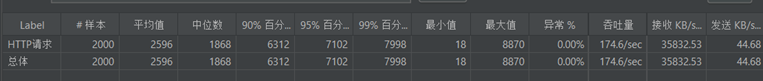
\includegraphics[width=0.8\textwidth]{redisa}
	\caption{优化前}
	\vspace{\baselineskip}
\end{figure}


采用redis后:
\begin{figure}[htbp]
	\centering
	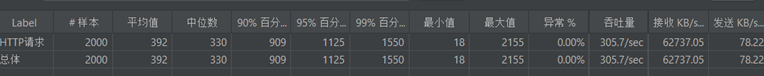
\includegraphics[width=0.8\textwidth]{redisb}
	\caption{优化后}
	\vspace{\baselineskip}
\end{figure}

可以看到吞吐量和延迟都有了很明显的优化效果

\section{数据库加密}

\subsection{背景}
在项目一,项目三,项目四中,数据库中的用户密码是明文存储的,这样一来,一旦数据库被攻破,用户的密码就会被泄露,造成不可挽回的损失。
于是,我们采取了数据库加密技术,以防止可能存在的攻击。

\subsection{传统哈希优化方法}
为了防止数据库被破解或请求被抓包而导致的用户隐私泄露问题,我们采取了新的数据库存储模式,即哈希加密存储方式,由前端本地进行哈希算法和加密,具体加密算法实现如下:

\begin{lstlisting}[basicstyle=\footnotesize]
public static String hashPassword(String password) {
	try {
		MessageDigest digest = MessageDigest.getInstance("SHA-256");
		byte[] hashBytes = digest.digest(password.getBytes(StandardCharsets.UTF_8));

		// Convert the byte array to a hexadecimal string
		StringBuilder hexString = new StringBuilder();
		for (byte hashByte : hashBytes) {
			String hex = Integer.toHexString(0xff & hashByte);
			if (hex.length() == 1) {
				hexString.append('0');
			}
			hexString.append(hex);
		}
		return hexString.toString();
	} catch (NoSuchAlgorithmException e) {
		e.printStackTrace();
	}
	return null;
}
\end{lstlisting}

采取了数据库加密算法之后,存储在数据库的密文形式如图\ref{fig:hash_sql}所示,可以看到整个密码都变成了无序的大小写字母的排列组合,变得更加安全可靠

\begin{figure}[htbp]
	\centering
	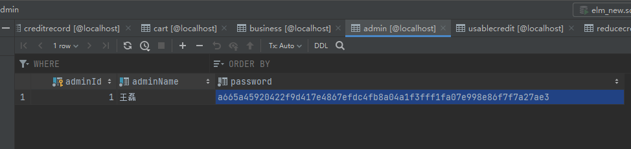
\includegraphics[width=0.8\textwidth]{hash_sql}
	\caption{哈希加密存储}
	\label{fig:hash_sql}
	\vspace{\baselineskip}
\end{figure}

但是这样的传统优化方式,也并不是绝对安全的,因为存在一种新的攻击方式,叫做彩虹表攻击。在计算机安全领域,密码通常以散列~(hash)的形式存储在数据库中,以防止未经授权的访问。然而,传统的哈希函数通常容易受到破解,因此需要更强大的密码保护机制。彩虹表攻击就是一种旨在破解散列密码的攻击技术之一。

\begin{figure}[htbp]
	\centering
	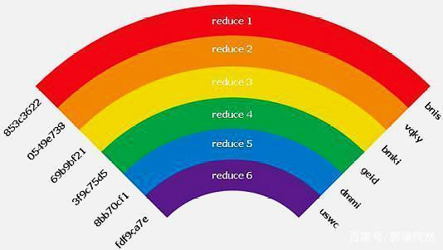
\includegraphics[width=0.8\textwidth]{rainbow}
	\caption{彩虹表}
	\vspace{\baselineskip}
\end{figure}

为了应对彩虹表攻击,我们采取了数据加盐加密的技术。

\subsection{加盐加密技术}

在密码学和信息安全领域,加盐加密技术是一种用于增强密码存储和传输的安全性的方法。
它在密码哈希过程中引入一个额外的随机值(盐),以使相同的明文密码在每次加密时都产生不同的散列值,从而增加破解密码的难度。

在本项目中,实现加盐加密算法的代码如下:

\begin{lstlisting}[basicstyle=\footnotesize]
public static final String SALT = "afhu&9TawdhYCbsad*dawdh1dawdjhaj";

public static String encodePassword(String strValue) throws NoSuchAlgorithmException {
	MessageDigest md5 = MessageDigest.getInstance("MD5");
	return Base64.encodeBase64String(md5.digest((strValue + CommonUtil.SALT).getBytes()));

}
\end{lstlisting}

同样地,在采取了加盐加密算法之后,数据库存储的密文形式如图\ref{fig:salt-sql}所示。

\begin{figure}[htbp]
	\centering
	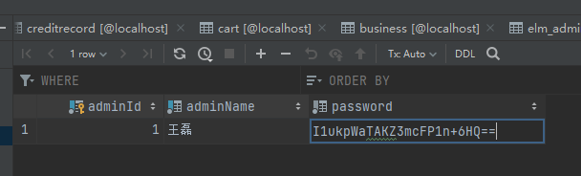
\includegraphics[width=0.8\textwidth]{salt_sql}
	\caption{加盐加密存储}
	\label{fig:salt-sql}
	\vspace{\baselineskip}
\end{figure}

\subsection{加密安全效果展示}

图\ref{fig:hack_1}为破解传统哈希算法的实例演示,图\ref{fig:hack_2}是加盐加密后,使用彩虹表攻击也无法成功破解数据库的密码。极大程度地提高了数据安全,保障了用户的个人隐私。

\begin{figure}[htbp]
	\centering
	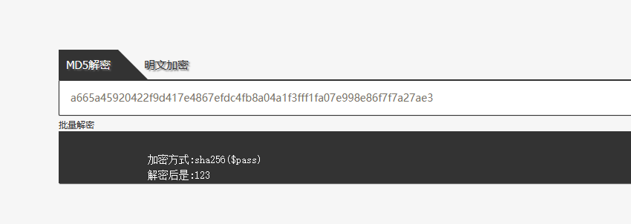
\includegraphics[width=0.8\textwidth]{hack_1}
	\caption{破解传统哈希算法}
	\label{fig:hack_1}
	\vspace{\baselineskip}
\end{figure}

\begin{figure}[htbp]
	\centering
	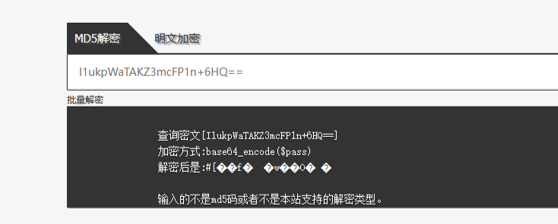
\includegraphics[width=0.8\textwidth]{hack_2}
	\caption{破解加盐加密算法}
	\label{fig:hack_2}
	\vspace{\baselineskip}
\end{figure}


\section{积分系统}
积分系统的设计参考了美团APP的米粒功能
\subsection{规则设计}
\subsubsection{积分获取}
\begin{enumerate}
	\item 签到获得积分,每日通过签到获得的积分上限为1次
	\item 消费时获得积分,订单金额按比例兑换为积分数量
	\item 充值时获得积分,将电子钱包的充值按比例转化为积分
\end{enumerate}
\subsubsection{积分消耗}
\begin{enumerate}
	\item 积分存在有效期,积分随着时间的增加自然减少
	\item 下单时可以通过消耗积分,来减少支付所需钱的数量
\end{enumerate}
\subsubsection{特殊的规则}
\begin{enumerate}
	\item 选择优先过期的积分进行消费
	\item 连续签到,节假日签到,特殊节日消费特殊商品等,有特殊的积分规则
\end{enumerate}

\subsection{数据库设计}

这里展示了积分规则的数据库图表,具体如下:

\begin{table}[htbp]
    \caption{可用积分表}
    \vspace{0.5em}\wuhao
    \begin{tabularx}{\hsize}{@{\extracolsep{\fill}}c c c}
    \toprule[1.5pt]
    字段名          & 数据类型  & 说明 \\ 
    \midrule[1pt]
    id      & int      & 主键id \\
    userId        & varchar  & 用户id \\
    recordId    & int  & 流水表记录id \\
    credit & int  & 积分值 \\
    createTime & datetime  & 创建时间 \\
    expiredTime       & datetime  & 过期时间 \\
    deleted   & int  & 过期标记 \\
    \bottomrule[1.5pt]
    \end{tabularx}
\vspace{\baselineskip}
\end{table}

\begin{table}[htbp]
    \caption{积分记录表(流水表)}
    \vspace{0.5em}\wuhao
    \begin{tabularx}{\hsize}{@{\extracolsep{\fill}}c c c}
    \toprule[1.5pt]
    字段名          & 数据类型  & 说明 \\ 
    \midrule[1pt]
    id      & int      & 主键id \\
    userId        & varchar  & 用户id \\
    ruleCode    & varchar  & 规则码 \\
    eventId & int  & 订单/充值id \\
    credit & int  & 积分值 \\
	createTime       & datetime  & 创建时间 \\
    expiredTime       & datetime  & 过期时间 \\
    \bottomrule[1.5pt]
    \end{tabularx}
\vspace{\baselineskip}
\end{table}

\begin{table}[htbp]
    \caption{积分规则表}
    \vspace{0.5em}\wuhao
    \begin{tabularx}{\hsize}{@{\extracolsep{\fill}}c c c}
    \toprule[1.5pt]
    字段名          & 数据类型  & 说明 \\ 
    \midrule[1pt]
    id      & int      & 主键id \\
    ruleCode    & varchar  & 积分规则码 \\
	type      & int      & 获取/消费 \\
	priority      & int      & 优先级 \\
	credit & int  & 积分值 \\
	formula & int & 公式 \\
	dalyCap & int & 日上限 \\
	totCap & int & 总上限 \\
	startTime       & datetime  & 开始时间 \\
    endTime       & datetime  & 结束时间 \\
	lifespan & int & 有限期 \\
	state & int & 启用/停用 \\
    \bottomrule[1.5pt]
    \end{tabularx}
\vspace{\baselineskip}
\end{table}

\begin{table}[htbp]
    \caption{积分扣除表}
    \vspace{0.5em}\wuhao
    \begin{tabularx}{\hsize}{@{\extracolsep{\fill}}c c c}
    \toprule[1.5pt]
    字段名          & 数据类型  & 说明 \\ 
    \midrule[1pt]
    id      & int      & 主键id \\
    userId        & varchar  & 用户id \\
    recordId    & int  & 流水表中消费积分记录id \\
    usableId & int  & 可用积分表中对应的记录id \\
    credit & int  & 积分值 \\
	createTime       & datetime  & 创建时间 \\
    expiredTime       & datetime  & 过期时间 \\
    \bottomrule[1.5pt]
    \end{tabularx}
\vspace{\baselineskip}
\end{table}

\subsection{接口设计}

\textbf{查询当前可用积分}

CreditController/queryAvailableCredit

参数:userId

返回值:int

功能:查找userId用户的所有可用积分

\textbf{查询积分流水}

CreditController/queryAllCredit

参数:userId

返回值:List(记录积分的数组)

功能:查找userId用户的所有专区或者消费的积分明细

\textbf{签到获得积分}

CreditController/earnCreditBySign

参数:userId,creditNum,ruleCode

返回值:int

功能:签到获得积分,每日通过签到获得的积分上限为1次

\textbf{查询签到可以获得的积分总数}

CreditController/queryEarningCreditBySign

参数:userId,ruleCode

返回值:int

功能:查找userId用户,在规则码为ruleCode的情况下,能够获取的积分总数

\textbf{查询支付可以获得的积分总数}

CreditController/queryEaringCreditByPaying

参数:userId,money,ruleCode

返回值:int

功能:给所有userId的用户查询支付money的钱可以获得多少积分

\textbf{支付后获得积分}

CreditController/earnCreditByPaying

参数:userId,orderId,creditNum,ruleCode

返回值:int

功能:让用户支付之后获得积分

\textbf{支付时抵扣积分}

CreditController/queryConsumingCreditByPaying

参数:userId,money,creditNum,ruleCode

返回值:creditNum,deductionMoney

功能:让用户在支付时使用积分做抵扣

\section{虚拟钱包系统}
参考美团APP的天天神券功能,制作了一个虚拟支付钱包。
\subsection{规则设计}
\subsubsection{电子钱包的创建}
\begin{enumerate}
	\item 用户同意时,主动创建一个钱包
	\item 商家需要主动与平台完成签约创建钱包
\end{enumerate}
\subsubsection{支付逻辑}
\begin{enumerate}
	\item 优先消耗积分支付
	\item 必须保证钱包扣款的线程安全
	\item 保障支付本身的事务性
\end{enumerate}
\subsection{具体实现}
在定义上,我们不仅采用了~pojo~层,还采用了~VO~层,其中,~pojo~层又叫~PO~,是面向数据库的,与其协同的对象分别为~Service~层和~Dao~层,放从数据库中直接拿出来的数据,没有任何逻辑实现,只有~getter~域~setter~方法,数据库的每一个字段都对应着~POJO~的一个属性。
~VO~是面向~Service~层与~Controller(Web)~层的,~VO~的数据是~POJO~中的数据加工后得到的,用于在~Web~页面上展示。

\begin{lstlisting}[basicstyle=\footnotesize]
package com.neusoft.elmboot.po;

public class VirtualWalletPo {
	private Integer walletId;
	private double balance;

	public VirtualWalletPo(){
		this.balance=0.00;
	}
	public VirtualWalletPo(Integer walletId,double balance){
		this.balance=balance;
		this.walletId=walletId;
	}
	public Integer getWalletId() {
		return walletId;
	}
	public double getBalance() {
		return balance;
	}
}
\end{lstlisting}

\begin{lstlisting}[basicstyle=\footnotesize]
package com.neusoft.elmboot.po;

public class VirtualWalletVo {
	private double money;
	private Integer walletId;
	private Integer inputWalletId;
	private Integer outputWalletId;
	private Integer orderId;
	private String userId;

	public String getUserId() {
		return userId;
	}

	public void setUserId(String userId) {
		this.userId = userId;
	}

	public Integer getOrderId() {
		return orderId;
	}

	public void setOrderId(Integer orderId) {
		this.orderId = orderId;
	}

	public Integer getInputWalletId() {
		return inputWalletId;
	}

	public Integer getOutputWalletId() {
		return outputWalletId;
	}

	public void setOutputWalletId(Integer outputWalletId) {
		this.outputWalletId = outputWalletId;
	}

	public void setInputWalletId(Integer inputWalletId) {
		this.inputWalletId = inputWalletId;
	}

	public double getMoney() {
		return money;
	}
	public void setMoney(double money) {
		this.money = money;
	}
	public Integer getWalletId() {
		return walletId;
	}
	public void setWalletId(Integer walletId) {
		this.walletId = walletId;
	}
}
\end{lstlisting}
		
\subsection{保障事务性}
在本项目中,为了保证钱包支付的事务性,我们采取了~synchronized~和自带线程安全的~cocurrentHashMap~来实现,具体为在操作线程钱进行加锁,来保证关于金钱操作的~ACID~事务性。
这里以~queryEarningCreditBySign~方法举例。

\begin{lstlisting}[basicstyle=\footnotesize]
@Override
public Integer queryEarningCreditBySign(String userId) {
	Integer ruleId = 1;
	String time = CommonUtil.getCurrentDate();
	String today = time.substring(0, time.indexOf(' ')).trim();
	int count = creditRecordMapper.todaySignRecord(userId, ruleId, today);
	SignCreditRule signCreditRule = null;
	synchronized (creditRuleMap) {
		signCreditRule = (SignCreditRule) creditRuleMap.getRule(ruleId);
		if (signCreditRule == null) {
			CreditRulePo creditRulePo = creditRuleMapper.getRule(ruleId);
			int credit = creditRulePo.getCredit();
			int lifeSpan = creditRulePo.getLifespan();
			int totCap = creditRulePo.getDailyCap();
			signCreditRule = new SignCreditRule(lifeSpan, credit, totCap);
			creditRuleMap.writeMap(ruleId, signCreditRule);
		}
	}
	CreditSystem creditSystem = new CreditSystemImpl();
	return creditSystem.queryEarningCreditBySign(count, signCreditRule);
}
\end{lstlisting}


\section{使用vue3}
此次项目中,我们放弃了原来的vue2,采用vue3进行前端开发,性能得到了显著的提升,具体优点如下:
\begin{enumerate}
	\item {diff算法的优化}:vue3新增了静态标记(patchflag),在Vue2中,每次更新diff,都是全量对比,Vue3则只对比带有标记的,这样大大减少了非动态内容的对比消耗.
	\item {hoistStatic静态提升}:vue2无论元素是否参与更新,每次都会重新创建然后再渲染。vue3对于不参与更新的元素,会做静态提升,只会被创建一次,在渲染时直接复用即可。
	\item {cacheHandlers事件侦听器缓存}:vue2中,绑定事件每次触发都要重新生成全新的function去更新;Vue3中,cacheHandlers是事件缓存对象,当cacheHandlers开启,会自动生成一个内联函数,同时生成一个静态节点。当事件再次触发时,只需从缓存中调用即可,无需再次更新。
	\item {ssr渲染}:渲染时,若存在大量静态内容,这些内容会被当作纯字符串推进一个buffer里面,即使存在动态的绑定,也会通过模版插值潜入进去。这样会比通过虚拟dmo来渲染的快上很多。
	\item {按需编译,体积比vue2更小}:在 Vue 3 中,通过将大多数全局API和内部帮助程序移至ES模块导出来,减小了框架。这使现代的打包工具可以静态分析模块依赖性并删除未使用的导出相关的代码。模板编译器还会生成友好的 Tree-shaking 代码,在模板中实际使用了该功能时才导入该功能的帮助程序。
	\item {支持多根节点组件}:在vue2中,不支持多根组件,当用户意外创建多根组件时会发出警告,而vue3中,组件可以有多个根节点。
\end{enumerate}

\section{使用AI技术设计一套简单的推荐算法}
\subsection{参考架构}
我们在考虑引入推荐功能时,参考了目前常见的~AI~推荐算法架构,如图\ref{fig:AI_1}所示。
\begin{figure}[htbp]
	\centering
	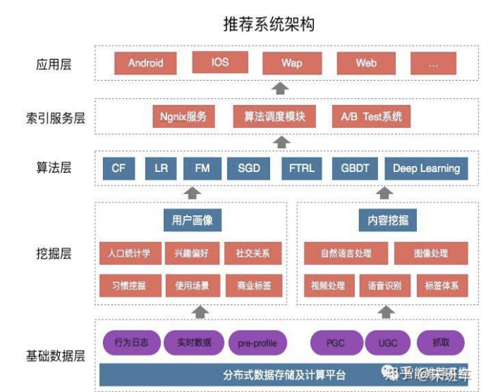
\includegraphics[width=0.8\textwidth]{AI_1}
	\caption{加盐加密存储}
	\label{fig:AI_1}
	\vspace{\baselineskip}
\end{figure}

\subsection{遇到的困难}
但在具体的操作过程中,由于受到诸多因素的影响,遇到了许多困难,比如:
\begin{enumerate}
	\item 数据量过少,算法层模型的效果不明显
	\item 应用层埋点过少,特征数过少,分类效果不佳
	\item 服务器性能差,无法承担大模型推理+数据挖掘+模型微调的常见推荐算法
	\item 基础数据层建设不完善,系统不完备,比如日志系统,账号系统,商家系统等数据量少。
\end{enumerate}
\subsection{算法设计}
算法逻辑实现:
\begin{enumerate}
	\item 优先推荐同标签里热度最高的商家
	\item 在相同标签内,相同热度商家中推荐id更小的商家
	\item 如果没有相同的标签,则推荐其他中热度最高的商家
\end{enumerate}
\subsection{算法实现}
实际在数据库中,使用了kmeans算法对商家的起送费与配送费进行数据分析,对商家提供的菜品种类和价格等进行了聚类,分类的结果如图\ref{fig:alg_3}所示,实际部署后,在数据库中体现的截图效果如图\ref{fig:alg_1}所示。在饿了么项目的实际展示中效果如下图\ref{fig:alg_2}所示
\begin{figure}[htbp]
	\centering
	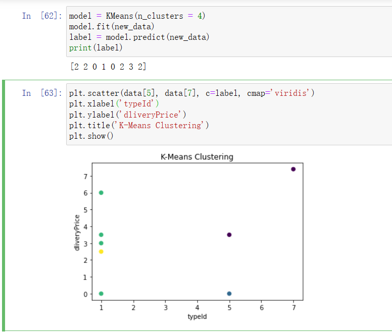
\includegraphics[width=0.8\textwidth]{alg_3}
	\caption{数据可视化}
	\label{fig:alg_3}
	\vspace{\baselineskip}
\end{figure}
\begin{figure}[htbp]
	\centering
	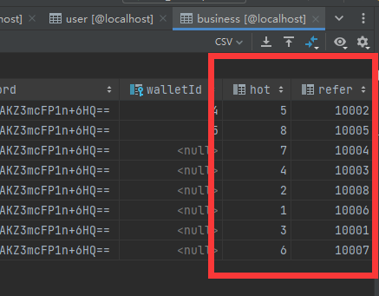
\includegraphics[width=0.5\textwidth]{alg_1}
	\caption{数据库处理}
	\label{fig:alg_1}
	\vspace{\baselineskip}
\end{figure}
\begin{figure}[htbp]
	\centering
	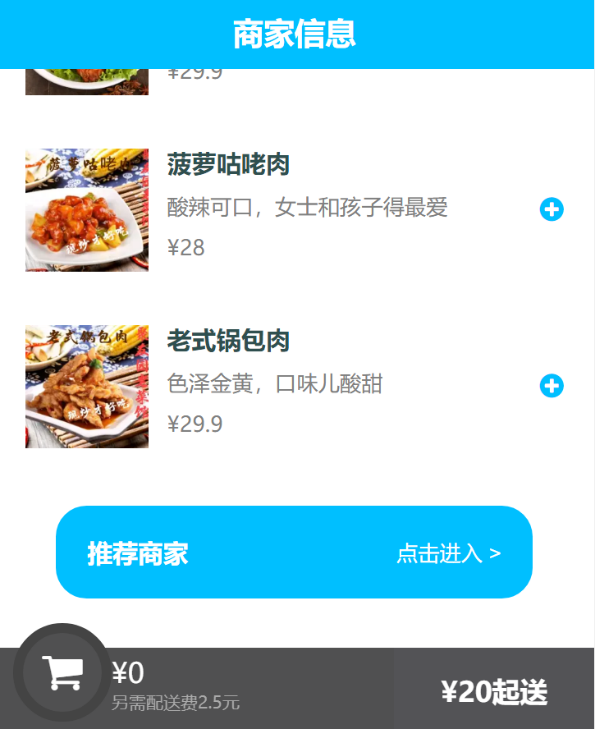
\includegraphics[width=0.5\textwidth]{alg_2}
	\caption{项目实际展示}
	\label{fig:alg_2}
	\vspace{\baselineskip}
\end{figure}